% (c) Copyright 2017 Josh Wright
\documentclass[12pt]{article}
\usepackage{verbatim}
% \usepackage{syntonly}
\usepackage{ragged2e}
\usepackage{geometry}
\usepackage{enumitem} % for longenum
\usepackage{setspace}
\usepackage{hyperref}
\usepackage{tabularx}
\usepackage{graphicx}
\usepackage{outlines} % for outline
\usepackage{paralist} % for compactitem (compact itemize)
\usepackage{multicol} % for multicolumn layout
\geometry{letterpaper, margin=0.4in, top=0.2in}
% \geometry{letterpaper, margin=0.5in, top=0.35in, left=1.5in}
\pagenumbering{gobble}
\begin{document}
\begin{spacing}{0.8}
%%%%%%%%%%%%%%%%%%
%% main section %%
%%%%%%%%%%%%%%%%%%
\begin{multicols*}{2}
\begin{flushleft}
\newlist{longenum}{itemize}{5}
\setlist[longenum,1]{nosep,leftmargin=0.2cm,labelwidth=0px,align=left,label=$\bullet$}
\setlist[longenum,2]{nosep,leftmargin=0.2cm,labelwidth=0px,align=left,label=$\ast$}
\setlist[longenum,3]{nosep,leftmargin=0.2cm,labelwidth=0px,align=left,label=-}
\setlist[longenum,4]{nosep,leftmargin=0.2cm,labelwidth=0px,align=left,label=$\cdot$}
\setlist[longenum,5]{nosep,leftmargin=0.2cm,labelwidth=0px,align=left,label=@}
% \begin{outline}[compactitem]
\begin{outline}[longenum]
%%%%%%%%%%%%%%%%%%%%
%% spacing config %%
%%%%%%%%%%%%%%%%%%%%
% just in case I need even more space
\newlength{\upspacelength}
\setlength{\upspacelength}{0px}
\newcommand{\upspace}{\vspace{\upspacelength}}
% section titles
\newcommand{\zzz}[1]{\upspace \0 \textbf{#1} }
% \newcommand{\zzz}[1]{\0 \hspace{-1.25in} \textbf{#1} \vspace{-10px} }
% makes second-level itemize bullets instead of dashes
% \renewcommand\labelitemii{\labelitemi}
% redefine the sub-headings to inject our space-saver
\let\oldOne\1\let\oldTwo\2\let\oldThree\3\let\oldFour\4
\renewcommand{\1}{\oldOne   \hspace{-6px}}
\renewcommand{\2}{\oldTwo   \hspace{-6px}}
\renewcommand{\3}{\oldThree \hspace{-6px}}
\renewcommand{\4}{\oldFour  \hspace{-6px}}
\small

\noindent ECEN454 Ref Sheet \hfill \textcopyright \space Josh Wright \today

\newcommand{\VDD}{V_{DD}}

\newcommand{\Vt}{V_{t}}
\newcommand{\Vtn}{V_{tn}}
\newcommand{\Vtp}{V_{tp}}

\newcommand{\Vg}{V_{g}}
\newcommand{\Vs}{V_{s}}
\newcommand{\Vd}{V_{d}}
\newcommand{\Vgn}{V_{gn}}
\newcommand{\Vsn}{V_{sn}}
\newcommand{\Vdn}{V_{dn}}
\newcommand{\Vgp}{V_{gp}}
\newcommand{\Vsp}{V_{sp}}
\newcommand{\Vdp}{V_{dp}}

\newcommand{\Vgs}{V_{gs}}
\newcommand{\Vgd}{V_{gd}}
\newcommand{\Vds}{V_{ds}}
\newcommand{\Vgsn}{V_{gsn}}
\newcommand{\Vgdn}{V_{gdn}}
\newcommand{\Vdsn}{V_{dsn}}
\newcommand{\Vgsp}{V_{gsp}}
\newcommand{\Vgdp}{V_{gdp}}
\newcommand{\Vdsp}{V_{dsp}}
% \newcommand{\V}{V_{}}
% \newcommand{\V}{V_{}}

\zzz{Metric Prefixes} \\
\begin{tabular}{|c c l l|}                                   \hline
peta  & P     & $10^{ 15}$ & \hfill 1 000 000 000 000 000 \\ \hline
tera  & T     & $10^{ 12}$ & \hfill     1 000 000 000 000 \\ \hline
giga  & G     & $10^{  9}$ & \hfill         1 000 000 000 \\ \hline
mega  & M     & $10^{  6}$ & \hfill             1 000 000 \\ \hline
kilo  & k     & $10^{  3}$ & \hfill                 1 000 \\ \hline
hecto & h     & $10^{  2}$ & \hfill                   100 \\ \hline
deca  & da    & $10^{  1}$ & \hfill                    10 \\ \hline
one   &       & $10^{ 0 }$ & \hfill       1 \hfill \hfill \\ \hline
deci  & d     & $10^{- 1}$ & 0.1                          \\ \hline
centi & c     & $10^{- 2}$ & 0.01                         \\ \hline
milli & m     & $10^{- 3}$ & 0.001                        \\ \hline
micro & $\mu$ & $10^{- 6}$ & 0.000 001                    \\ \hline
nano  & n     & $10^{- 9}$ & 0.000 000 001                \\ \hline
pico  & p     & $10^{-12}$ & 0.000 000 000 001            \\ \hline
femto & f     & $10^{-15}$ & 0.000 000 000 000 001        \\ \hline
\end{tabular}

\zzz{De Morgan's Laws}
  \1 $\overline{AB}=\overline {A}+\overline{B}$
  \1 $\overline{A+B}=(\overline{A})(\overline{B})$

\zzz{Silicon}
  \1 Si
  \1 P-type:
    \2 doped with material to remove electrons (add electron holes), usually Boron (B), Aluminum (Al), or Gallium (Ga)
  \1 N-type:
    \2 doped with material to add electrons, usually Antimony (Sb), Arsenic (As), or Phosphorous (P)
  \1 Silicon dioxide: SiO$_2$
  \1 Polysilicon is just silicon without the crystal structure

\zzz{Transistors}
  \1 pMOS:
    \2 has the bubble
    \2 on when input is 0, off when input is 1
  \1 nMOS
    \2 no bubble
    \2 on when input is on, off when input is off
  \1 CMOS: when you combine a nMOS and pMOS network together to make a gate, where one is the compliment of the other
  \1 $V_t$: Threshold voltage. Nominal voltage below which the transistor is off
    \2 below as in closer to 0, not less
    \2 $V_t>0$ for nMOS, $V_t<0$ for pMOS
    \2 this is compared to the gate to source voltage, $V_{gs}$
  \1 regions: (for nMOS)
    \2 accumulation: gate is negatively charged, attracts positive voids in p-substrate, which block flow in the channel
    \2 depletion: small positive charge on gate repels positive voids from channel, forming a depletion below the gate
    \2 inversion: higher positive charge ($>V_t$) is applied to gate, attracting electrons to the channel and allowing flow

\zzz{D Flip Flop vs Latch}
  \1 latch is level triggered
  \1 flip flop is edge triggered

\zzz{Fabrication}
  \1 n-well: use diffusion or ion implantation
  \1 positive lithography: expose to UV where you want to remove material
  \1 negative lithography: expose to UV where you want to keep material



% lecture 4
\zzz{Stick Diagram vs Boolean Function}
  \1 TODO
  \1 there is more than one way of making a stick diagram for an expression
    \2 stuff in series could be in different order, for instance
  \1 if you do it manually, you need to check it with tools:
    \2 LVS: Layout Vs Schematic
    \2 DRC: Design Re-Check
    \2 These aren't really needed for designs automatically generated from verilog code, because of course that's correct

\zzz{Lithography}
  \1 the process of printing onto a chip at nanometer scale
  \1 generally uses UV light, wavelength around 150nm
    \2 must use fancy tricks to make 10nm features with 150nm light
    \2 would be nice to use even lower wavelength X-rays, but those are hard to focus
  \1 negative lithography: use the lithography mask to cover what you want to keep.
  \1 positive lithography: mask what you want to remove
  \1 a lens is used to focus the light
    \2 ideally, want a point source for the light, but that is not practical
    \2 Optical Proximity Effect: what happens when your focus from the lens is not just right
    \2 results in rounded corners, inaccurate critical dimensions, and shorter wire ends
    \2 can use Optical Proximity Correction to fix:
    \\ basically over-emphasize all the features, and/or add extra lines at outset

\zzz{MOS transitive $I$-$V$ Characteristics and Parasitics}
  \1 $I$-$V$: current-voltage relationship
  \1 Transistors are not really ideal switches, they have 3 zones of operation: cutoff, linear, saturation
  \1 definitions:
    \\ $V_{gs}$: voltage gate to source
    \\ $V_{gd}$: voltage gate to drain
    \\ $V_{ds}$: voltage source to drain (across the channel)
    \\ $V_t$: critical voltage at which transistor is saturated
    \\ channel: space between the source and drain, where the electrons flow
  \1 remember that the gate is insulated from the area under it by a thin layer of Silicon Dioxide (SiO$_2$)
  \1 by convention, the source is the terminal at lower voltage
  \1 \textbf{cutoff}:
    \2 when $V_{gs}<0$
    \2 electrons on the gate attract positive voids in the silicon below, and inhibit current flow. Therefore, the transistor is closed.
    \2 $I_{ds}=0$
  \1 \textbf{linear}:
    \2 $V_{gs}>V_t, V_{gd}=V_{gs}, V_{ds}=0$
    or $V_{gs}>V_t, V_{gs}>V_{gd}>V_t, 0<V_{ds}<V_{gs}-V_t$
    \2 $I_{ds}$ linearly proportional to $V_{ds}$
    \2 channel of electrons forms, allowing current to flow
  \1 \textbf{saturated:}
    \2 $V_{gs}>V_t, V_{gd}<V_t, V_{ds}>V_{gs}-V_t$
    \2 channel pinches off due to electrons attracting to source
    \2 $I_{ds}$ is independent of $V_{ds}$
\zzz{capacitor effect}
  \1 gate and channel can have a parallel plate capacitor effect, with the thin layer of SiO$_2$ acting as the insulator
  \1 $C=\frac{Q}{V}=\epsilon_{SiO_2}wl/t_{SiO_2}, V = V+{gc}-V_t=(v_{gs}-V{ds}/2)-V_t$
    \2 $l,w$: length, width of section of gate above channel
    \2 $\epsilon_{SiO_2}$: permittivity of SiO$_2$ layer
    \2 $t_{SiO_2}$: thickness of SiO$_2$ layer
  \1 general capacitance per unit area: $C_{ox}=\frac{\epsilon_{ox}}{t_{ox}}$
    \2 $\epsilon_{ox}$: permittivity of oxidation layer
    \2 $t_{ox}$: thickness of oxidation layer
  \1 carrier velocity: velocity of the electrons?
    \2 proportional to the electric field running horizontally between source and drain
    \2 $v=\mu E, E=V_{ds}/L, t=L/v=L/(\mu E)=L/(\mu\frac{V_{ds}}{L})$
    \\ $\mu$: mobility. electrons move about twice as fast as positive voids
    \\ $L$: length of channel
  \1 actual velocity of electrons is the speed of light, but they don't travel in a straight line, they travel atom-to-atom
    \2 this slowdown is called the \textbf{scattering} effect
\zzz{Shockley model of transistor}
  \1 $V_{dsat}=V_{gs}-V_t$
  \1 1st order model: $\beta=\mu C_{SiO_2}\frac{w}{l}$
  \begin{tabular}{l l l}
  $V_{gs} < V_t     $ & $I_{ds}=0$                                        & cutoff  \\
  $V_{ds} < V_{dsat}$ & $I_{ds}=\beta(V_{gs}-V_t-\frac{V_{ds}}{2})V_{ds}$ & linear \\
  $V_{ds} > V_{dsat}$ & $I_{ds}=\frac{\beta}{2}(V_{gs}-V_t)^2$            & saturation  \\
  \end{tabular}
  \1 Must be able to derive this model on exam!

\zzz{Non-Ideal $I$-$V$ Effects}
  \1 velocity saturation (due to scattering)
    \2 also called short channel effect
    \2 this is hard to make into a mathematical formula
  \1 sub-threshold leakage, junction leakage, gate tunneling
  \1 \textbf{Body Effect}
    \2 affected by $V_{sb}$: voltage of the p-substrate (which should be ground)
    \2 $V_t=V_{t0}+\lambda(\sqrt{|-2\phi_F+V_{sb}|}-\sqrt{|-2\phi_F|})$
      \3 $V_{t0}$: threshold without body bias
      \3 $\phi_F$: Fermi potential
        \4 negative for nMOS, positive for pMOS
      \3 $\lambda$: body effect coefficient
        \4 positive for nMOS, negative for pMOS (reversed)
    \2 generally fixed/caused by biasing
    \2 Forward Body Bias (FBB):
      \3 $V_{sb}<0, V_t<V_{s0}$
      \3 gates switch faster, but leak more current
    \2 Reverse Body Bias (RBB):
      \3 $V_{sb}>0, V_t>V_{s0}$
      \3 gates switch slower, but consume less power (because less leakage)
  \1 \textbf{Temperature}
    \2 higher temperature means higher electron mobility, more leakage, and threshold decreases
  \1 \textbf{Diffusion Capacitance}
    \2 capacitance on the source/drain: $C_{sb}, C_{db}$
      \3 source/drain are diffusion nodes
      \3 $C$ is comparable to $C_g$ (gate) for connected nodes, $\frac{1}{2}C_g$ for unconnected
      \3 (depends on process)
    \2 this is the capacitance we care most about (because we must fill it every time the gate switches?)
    \2 if two capacitors share a source/drain, that reduces diffusion capacitance (reducing this is a good thing)
    \2 also, you can remove unconnected diffusion spots
% end lecture 4

% lecture 5
\zzz{DC Response}
  \1 example: inverter
  \1 must settle to $I_{dsn}=|I_{dsp}|$
  \1 $V_{tn}, V_{tp}$: threshold voltages for nMOS and pMOS 
    (defined in Non-Ideal $I$-$V$ Effects)
  \1 $V_{in}=V_{DD} \rightarrow V_{out}=0$, $V_{in}=0 \rightarrow V_{out}=V_{DD}$
  \1 nMOS
    \2 $V_{gsn}=V_{in}, V_{dsn}=V_{out}$
    \2 cutoff:    $V_{in}<V_{tn}$
    \2 linear:    $V_{in}>V_{tn}, V_{out}<V_{in}-V_{tn}$
    \2 saturated: $V_{in}>V_{tn}, V_{out}>V_{in}-V_{tn}$
  \1 pMOS
    \2 $V_{gsp}=V_{in}-V_{DD}, V_{dsp}=V_{out}-V_{DD}, T_{tp}<0$
    \2 cutoff:    $V_{in}>V_{DD}+V_{tp}$
    \2 linear:    $V_{in}<V_{DD}+V_{tp}, V_{out}>V_{in}-V_{tp}$
    \2 saturated: $V_{in}<V_{DD}+V_{tp}, V_{out}<V_{in}-V_{tp}$
  \1 to calculate actual output voltage, balance $I_{dsn}=I_{dsp}$ (easiest to do graphically)
    \2 end up with a graph of $V_{out}$ as function of $V_{in}$
    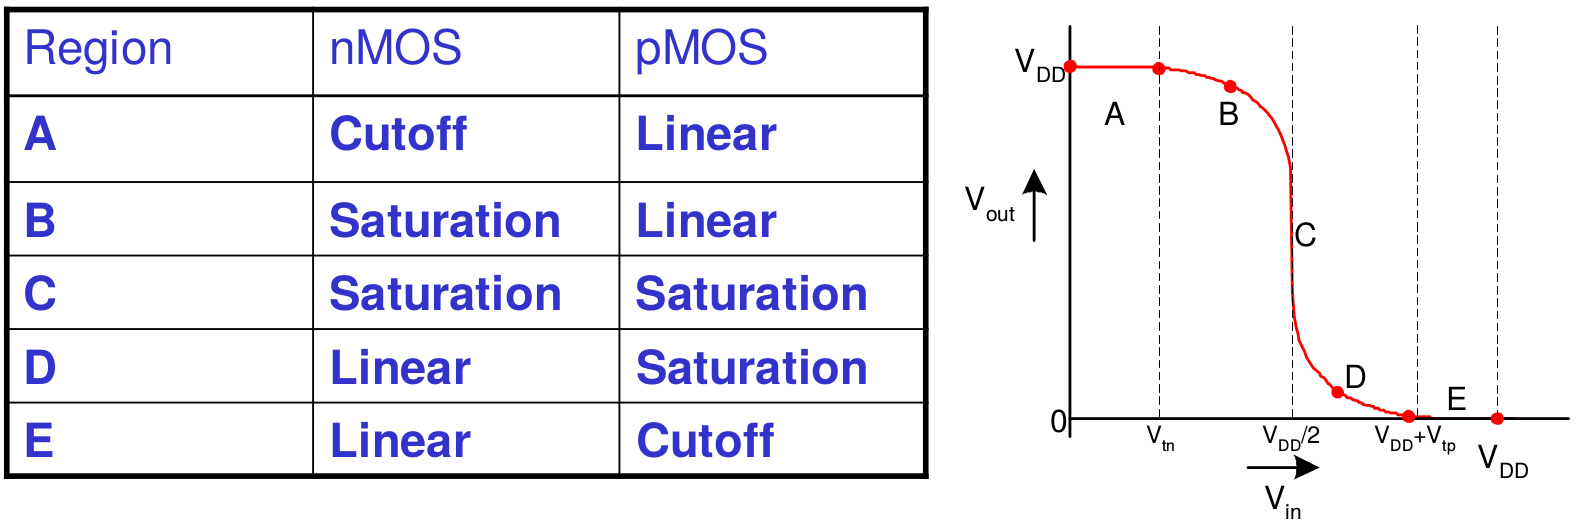
\includegraphics[width=\columnwidth]{ecen454/DC__response_Vo_Vi_nMOS_pMOS.png}
    \2 don't want to switch nMOS and pMOS because then nMOS would saturate at far end of graph (and vice versa for pMOS)
    \2 horizontal position of graph can be varied by tuning $\beta_p / \beta_n$
      \3 called beta ratio, or skewed gate
      \3 $\beta_p / \beta_n>1 \rightarrow$ right, $\beta_p / \beta_n\rightarrow$ left
    \2 unity gain slope: part of response graph where the slope is $-1$
      \3 want to tune $\beta_p / \beta_n$ to put logic levels at these regions to maximize noise margins
    \2 Noise Margins:
      \3 $NM_H=|V_{OH}-V_{IH}|, NM_L=|V_{OL}-V_{IL}|$
      \3 that's just the higher/lower of the two axes

\zzz{Transient Analysis}
  \1 for instance, find step response of gate to determine rise time.
  \1 rise/fall delay: time from when $V_{in}$ crosses $\frac{V_{DD}}{2}$ to when $V_{out}$ crosses it
  \1 rise/fall time: (of $V_{in}$ or $V_{out}$): time for that signal to go from $0.1V_{DD}$ to $0.9V_{DD}$ (or reverse)
  \1 TODO many equations and such for inverter step response (from slides)
  \1 TODO pass transistors (form slides)

\zzz{Pass Transistors}
  \1 for nMOS trying to pass $\VDD$ or pMOS trying to pass 0
  \1 nMOS can pull no higher than $\VDD-\Vtn$ if $\Vg=\VDD$
    \2 more generally, $\Vg-\Vtn$
    \2 called degraded 1
  \1 pMOS can pull no lower than $|\Vtp|$
% end lecture 5

% lecture 6
\zzz{Delay}
  \1 generally estimated with RC models
  \1 effective R for transistors and C of gate caps and parasitic caps
  \2 exactly what parasitic caps depends on exact layout (which stuff is shared between transistors)
  \1 width:
    \2 C proportional to width
     (approx 2 fF/$\mu$m)
    \2 R inversely proportional to width
      (approx 6k$\Omega$*$\mu$m)
    \2 TODO unity transistors
  \1 use effective resistance in RC model: $I_{ds}=V_{ds}/R$
    (just good enough for a RC model, not for current at arbitrary time)
  \1 find delay of circuit
    \2 decompose to RC model (take into account widths of each transistor)
      \3 replace transistors with resistors
      \3 add parasitic caps
    \2 add together all R and C's to get delay
  \1 Elmore Delay:
    \2 ON transistors look like resistors, so pullup/pulldown network is modeled as RC ladder
    \2 $t = \sum_{i\in nodes} R_{i-to-source}C_i$
    $= R_1C_1 + (R_1+R_2)C_2+\ldots+(R_1+\ldots+R_n)C_n$
    

\zzz{Power Estimation}




\end{outline}
\end{flushleft}
\end{multicols*}
\end{spacing}
\end{document}
